% h = here (try to place the figure exactly where the code appears)
% t = top (place it at the top of a page)
% b = bottom (place it at the bottom of a page)
% p = page of floats (place it on a separate page with just figures/tables)
% ! = override restrictions (e.g., \begin{figure}[!ht] tells LaTeX to try harder to place it here)
In this section, we present the results of our analyses. First, we show the baseline domain filtering analysis of all the parental control systems, providing insights into how each system blocks domains. Next, we show their overall blocking behavior and examine their blocking mechanisms by category, showing how each system handles different types of content.
 
\subsection{Baseline Domain Filtering} \label{sec:results-baseline}
%\todo[inline]{Ale: Do we report somewhere that we did not consdier dns over https?}
As outlined in Section \ref{sec:methodology}, we analyzed the PCAPs of each router’s LAN and WAN connections to assess their parental control mechanisms. We established a baseline for blocking behavior by testing HTTPS connections both with and without parental control. Our findings show that the routers do not apply HTTPS-based filtering. Instead, they rely on DNS-based filters, each using a different approach.

TP-Link, for instance, implements a basic keyword-based filter mechanism, blocking DNS queries that contain user-defined keywords. Our packet capture analysis confirms this behavior: such DNS queries are visible on the LAN connection between the computer and the router, but are absent on the WAN connection between the router and the Internet. This suggests that the router intercepts and drops these DNS requests before they are forwarded to the external network.
In contrast, Netgear uses a more advanced approach.
It intercepts DNS queries and validates them against an internal API at \emph{\url{https://urldb.meetcircle-netgear.co}}.
If a domain is flagged as inappropriate or harmful, the router blocks access by responding with an IP address from the \emph{10.123.0.0/16} range.
Additionally, this router allows users to fine-tune blocking with four protection levels: Child, Teen, Adult, and None.
ASUS, on the other hand, redirects all DNS queries to Cloudflare for Families (\emph{IP address: 1.1.1.3}) when parental control is enabled. 
If a domain is deemed inappropriate, Cloudflare for Families returns the IP address \emph{0.0.0.0} instead of the correct address, blocking access by preventing the resolution of the domain.
Based on our analysis, the decision on whether a domain is allowed or not is made entirely by the Cloudflare service.

Regarding the Norton software, our initial approach was similar to the one used for the routers, capturing PCAPs using Wireshark during browsing sessions. However, Norton was not suited for this type of measurement. We observed inconsistent signs of activity, such as failed TLS handshakes, or unexplained delays. These artifacts were not regular or reliable enough to support a large scale measurement. For this reason, we developed an alternative detection strategy. After exploring several approaches, including monitoring the behavior of the browser extensions installed by Norton, we settled on a curl-based script that determine if a domain is blocked by analyzing its HTML content. Specifically, we look for known indicators of a Norton block page, such as the presence of the term “NortonLifeLock” and references to the logo file used in the block page.

Finally, for the DNS resolvers, OpenDNS FamilyShield and DNS.eu Kids, we send a DNS query and record the response for domains from the Tranco list. A domain is classified as blocked if the response is empty (for DNS.eu Kids) or if it contains a known block IP address (\emph{146.112.61.106} for OpenDNS).


%\todo[inline]{Ale: The takeways are not clear to mme: they seem to mix the mechanisms used by routers/resovers/software to block access to inappropriate websites with the mechanisms we used to study them.}
\textit{Key takeaway: Routers and DNS resolvers implement parental control systems through DNS-based filters, involving user-defined keywords, external services, or redirecting to a blocking page. In contrast, software-based systems require analyzing the HTML content of the webpage. This attests the diversity of blocking methodologies among parental controls.}
%=======
%\textit{Key takeaway: Routers and DNS resolvers implement parental control systems through DNS-based filters, involving user-defined keywords, external services, or redirecting to a blocking page. In contrast, software-based systems require analyzing the HTML content of the webpage. This attests the diversity of blocking methodologies among parental controls.}
%>>>>>>> 4795dab (results and discussion)

\subsection{Overall Blocking Behavior}  \label{sec:results-overallblocking}

After analyzing the blocking mechanisms of each system, we evaluated the total number of domains blocked to assess their effectiveness in filtering inappropriate content. As shown in Figure~\ref{fig:blocked_domains}, Norton blocks 322,870 domains, significantly more than any other system, followed by DNS.eu with 132,045 blocked domains. %%%Check if it works like this
\begin{figure}
    \centering
    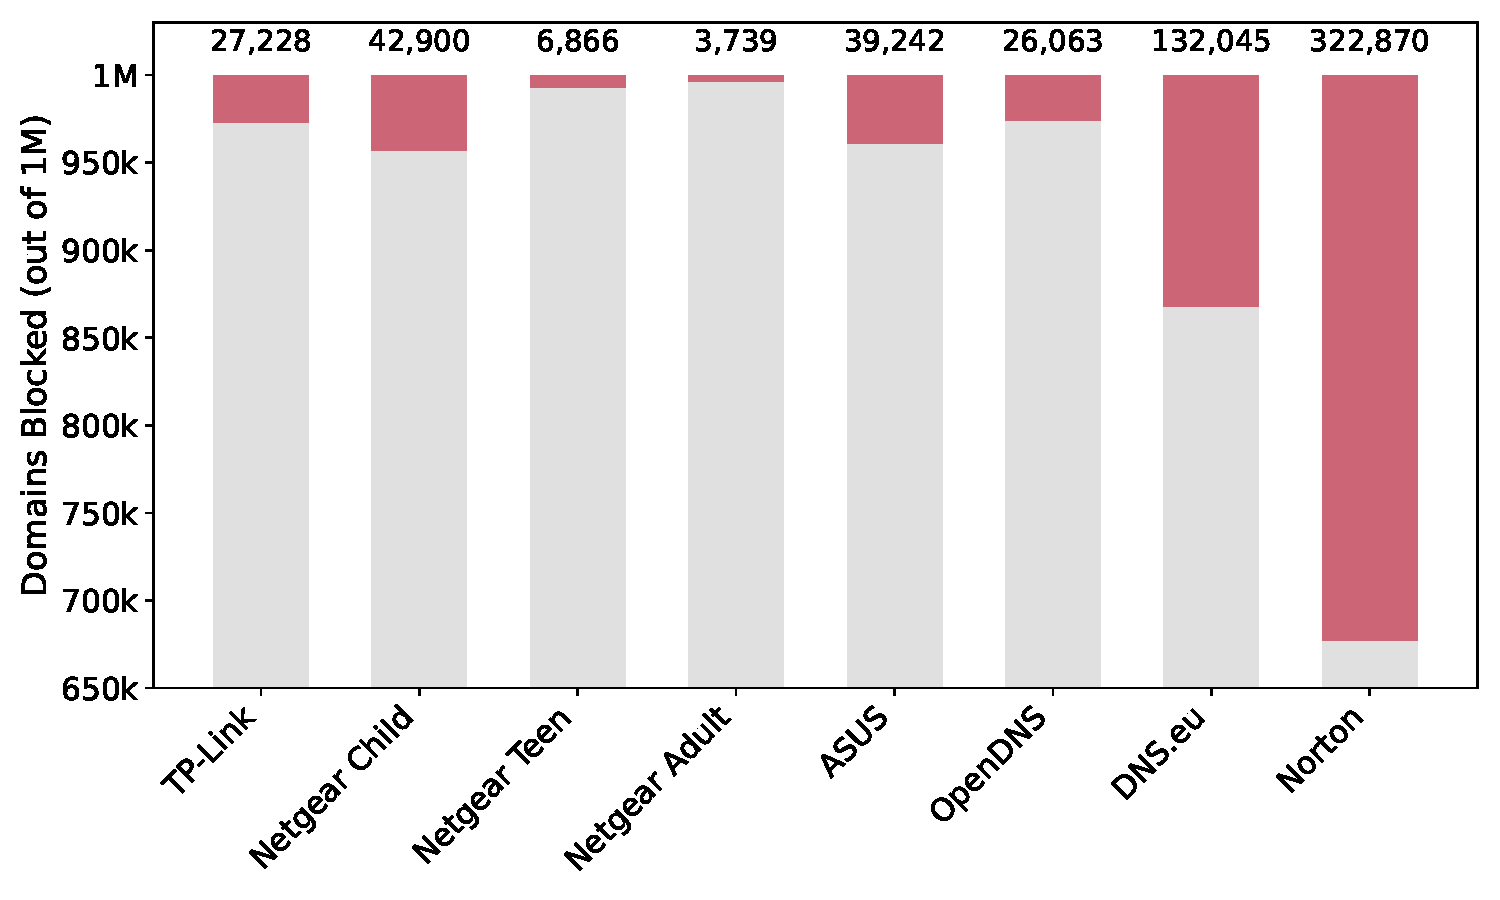
\includegraphics[width=0.85\columnwidth]{Images/Results/blocked_domains_per_tool.pdf}
    \caption{Total number of domains blocked by each parental control system.}
    \label{fig:blocked_domains}
\end{figure}
Netgear’s blocking behavior varies significantly depending on the setting. For example, in the Adult setting, it blocks fewer than 4k domains, while in the Child setting, it blocks over 10 times as many (42,900). The teen setting, on the other hand, blocks 6,866 domains.
The variation is expected, as these configurations are designed for different use cases. However, we also expected less variation between the Child and Teen settings than between the Teen and Adult settings, as both Child and Teen options are supposed to filter content for younger users, while the Adult option is typically less restrictive.
In comparison, ASUS blocks a closer number of domains (39,242) to the Netgear's child setting. TP-Link, which allows users to specify keywords to block, blocks approximately 27,228 domains, more than OpenDNS that blocks approximately 26,000 domains. As a result, OpenDNS blocks the fewest domains among the systems evaluated, excluding Netgear’s Teen and Adult filters.

\begin{table*}[htbp]
    \centering
    \resizebox{\textwidth}{!}{
    \begin{tabular}{lcccccccc}
    \toprule
    \textbf{Category (Total)} & \textbf{TP-Link} & \textbf{Netgear Child} & \textbf{Netgear Teen} & \textbf{Netgear Adult} & \textbf{ASUS} & \textbf{OpenDNS} & \textbf{DNS.eu} & \textbf{Norton} \\
    \midrule
    Business and Industry (188448) & 0.3\% & 1.7\% & 0.1\% & 0.1\% & 0.3\% & 0.1\% & 7.6\% & 17.8\% \\
    Ecommerce/Shopping (87612) & 0.4\% & 4.7\% & 0.1\% & 0.1\% & 0.5\% & 0.1\% & 2.3\% & 17.2\% \\
    Technology (61398) & 0.3\% & 2.5\% & 0.2\% & 0.2\% & 0.6\% & 0.2\% & 8.2\% & 23.5\% \\
    Education and Research (49041) & 0.2\% & 2.8\% & 0.1\% & 0.1\% & 0.4\% & 0.0\% & 6.8\% & 12.7\% \\
    \textbf{Adult Content (33368)} & \textbf{27.7\%} & \textbf{5.0\%} & \textbf{5.6\%} & \textbf{6.3\%} & \textbf{63.8\%} & \textbf{73.5\%} & \textbf{70.5\%} & \textbf{74.5\%} \\
    News and Media (30659) & 0.5\% & 28.2\% & 0.2\% & 0.1\% & 0.2\% & 0.1\% & 2.3\% & 12.7\% \\
    Entertainment (30481) & 0.5\% & 6.1\% & 0.4\% & 0.2\% & 5.0\% & 0.6\% & 4.9\% & 24.8\% \\
    Fitness and Medicine (29054) & 0.4\% & 13.4\% & 0.1\% & 0.0\% & 0.6\% & 0.0\% & 4.4\% & 15.6\% \\
    Government and Law (24735) & 0.2\% & 28.5\% & 0.1\% & 0.1\% & 0.1\% & 0.0\% & 11.2\% & 6.2\% \\
    Travel (21535) & 0.7\% & 1.2\% & 0.2\% & 0.0\% & 0.1\% & 0.1\% & 3.8\% & 9.4\% \\
    \midrule
    \multicolumn{9}{c}{\textellipsis} \\
    \midrule
    \textbf{Gambling (20846)} & \textbf{16.9\%} & \textbf{3.7\%} & \textbf{4.4\%} & \textbf{0.4\%} & \textbf{0.9\%} & \textbf{0.2\%} & \textbf{13.9\%} & \textbf{75.3\%} \\
    \textbf{Hate/Discrimination (152)} & \textbf{0.7}\% & \textbf{19.1\%} & \textbf{9.2\%} & \textbf{0.7}\% & \textbf{10.5\%} & \textbf{7.2\%} & \textbf{13.8\%} & \textbf{46.1\%} \\
    \textbf{Terrorism (11)} & \textbf{0.0}\% & \textbf{18.2\%} & \textbf{27.3\%} & \textbf{0.0}\% & \textbf{54.5\%} & \textbf{0.0}\% & \textbf{18.2\%} & \textbf{36.4\%} \\
    \bottomrule
    \end{tabular}}
    \vspace{0.5\baselineskip} 
    \caption{Percentage of domains blocked by each parental control system, for the most frequent categories in the Tranco list and the four sensitive categories.}
    \label{tab:blocked_categories}
\end{table*}

To further understand the nature of this blocking, we also examined the ranking of the blocked domains in the Tranco list, specifically assessing whether the systems prioritize blocking higher-ranked and potentially more popular domains.
This is important because blocking popular domains may have a greater impact on real-life user experience and exposure to content compared to blocking low-traffic sites.

Figure~\ref{fig:cdf_blocked_domains} shows the cumulative distribution function of blocked domains across the Tranco Top 1 million list. The logarithmic scale is used to highlight differences in blocking behavior across domains with different popularity levels.
The x-axis represents the domain rank, from most to the least popular, while the y-axis shows the cumulative number of blocked domains up to each rank, with the axis ending at the total of one million domains.



Netgear Child shows the highest concentration of blocked domains in the early ranks, with 50\% of its blocked domains appearing within the top 31\% of the Tranco list (rank 310,472), and 90\% reaching rank 826,542. This suggests that, despite its limited overall coverage, Netgear Child prioritizes blocking more popular domains. Similarly, Netgear Adult follows a comparable trend, with 50\% of its blocked domains reaching rank 329,750.
In contrast, Netgear Teen shows a more gradual distribution, with 50\% of its blocked domains appearing only by rank 472,049. This suggest that its filtering is more spread out across the ranking, giving less emphasis on popular domains compared to the other Netgar configurations.
In contrast, TP-Link shows a relatively flat progression, reaching 50\% of its blocked domains only by rank 629,440, and 90\% by rank 952,000. This pattern is not due to an inherent filtering policy but reflects the limitations of the keyword-based blocking mechanism. Since domains are blocked only if their names contain a blocklist term, this approach disproportionately affects lower-ranked or obscure domains, where such terms are more likely to appear.
Norton, despite its much larger blocking volume, shows a more gradual rise: half of its blocked domains appear by rank 650,143, and 90\% by 930,832. 
DNS.eu, OpenDNS  and ASUS reach the 50\% thresholds at ranks 430,748, 459,953 and 480,093 respectively, around middle of the Tranco list, indicating a more balanced focus between popular and unpopular domains.
On average, across all eight systems, 50\% of blocked domains appear by rank 470,331, and 90\% by 886,945, indicating that most tools concentrate their blocking in the lower half of the Tranco list.

%\textcolor{red}{Norton stands out with a steep and early curve, indicating that it blocks a large number of domains across the entire ranking spectrum, including many highly ranked sites. DNS.eu and OpenDNS follow a similar pattern, though with a smaller total volume, still focusing their blocking on both popular and mid-ranked domains.
%TP-Link, using keyword filtering, shows a relatively flat CDF with only occasional steps, confirming that its blocking is sparse and not biased toward high-ranking domains. 
%This is expected, keyword-based blocking tends to affect niche or less popular domains, rather than well-known, high-traffic sites with specific, proprietary domain names.
%Netgear, across all three configurations, shows very limited blocking throughout the ranking. 
%The curves for the Adult, Teen, and Child settings remain nearly flat, indicating that not only do they block few domains overall, but also fail to prioritize domains with higher visibility or traffic. 
%This further reinforces the earlier observation that Netgear's parental control features do not effectively target the most prominent or potentially impactful domains.
%Overall, the CDF reinforces the pattern observed so far: 
%DNS-based systems and Norton offer broad, visible filtering, while router-based tools are either too narrow in scope or fail to block inappropriate content even when it appears in popuar domains.}

\textit{Key takeaway: Among the different solutions, we observe a large variability in the number of blocked domains with variations in the range of 300k to 7k, which raise questions about the effectiveness of these solutions.}

\subsection{Domain Blocking Across Categories} \label{sec:results-categories}
%Netgear is the only system that provides distinct filtering levels: Child, Teen, and Adul. To explore how the blocking is applied across these levels, we trace how individual domains are classified across these settings to assess the logical consistency of its filtering features.



\begin{figure}[t]
    \centering
    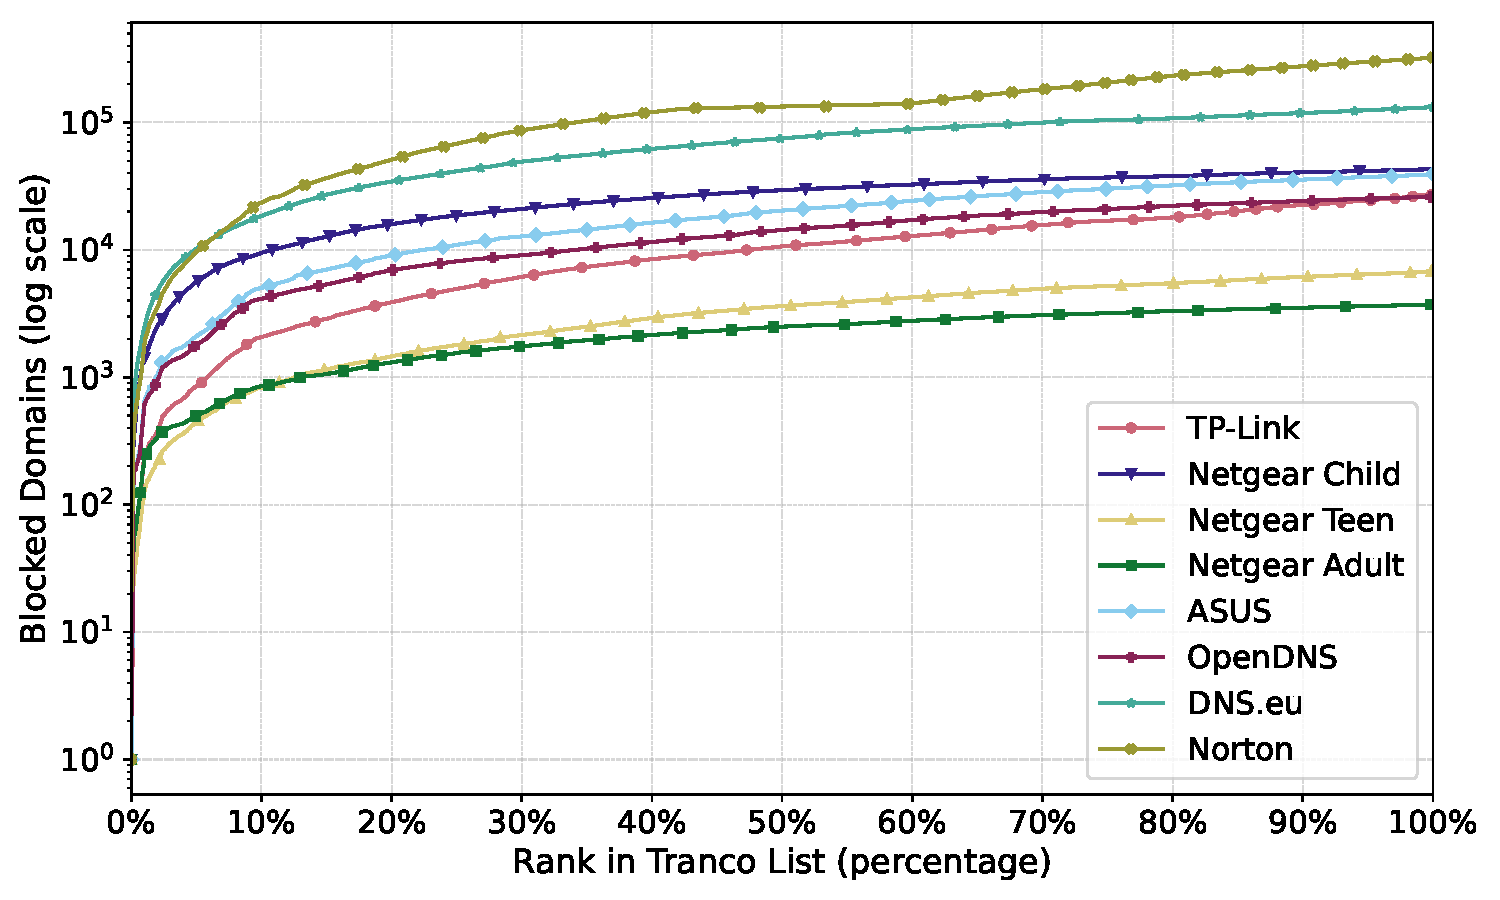
\includegraphics[width=0.85\columnwidth]{Images/Results/cdf_blocked_domains_log.pdf}
    \caption{Cumulative Distribution of Sensitive Domains Across the Tranco Top 1 million.}
    \label{fig:cdf_blocked_domains}
\end{figure}

To better understand the types of content most frequently blocked by each system, we evaluated the proportion of blocked domains across various content categories. We calculated the ratio of blocked domains in each category to the total number of domains in that category, as shown in Table~\ref{tab:blocked_categories}. Several notable patterns emerge, revealing strong differences in filtering priorities. We observe that systems like OpenDNS, DNS.eu, and Norton block a high percentage of domains across the sensitive category \emph{Adult Content}, with blocking rates of 73.5\%, 70.5\% and 74.5\% respectively. Additionally, Norton stands out as the system that blocks over 73\% of domains in the \emph{Gambling} category and achieves the highest blocking rates in \emph{Hate/Discrimination} and \emph{Terrorism}, further confirming its overall stricter filtering policy. 
However, on the other hand, Norton applies its broad filtering even to non-sensitive domains, blocking over 15\% of \emph{Education}, \emph{Technology}, and \emph{Business and Industry} sites, raising concerns about overblocking.

In contrast, router-based systems tend to block fewer domains and show more variability in their filtering across categories.
Notably, despite being the most restrictive among Netgear's settings, the Child configuration performs poorly in inappropriate categories, blocking only 5.0\% of \emph{Adult Content} and 3.7\% of \emph{Gambling} domains. Additionally, \emph{Hate/Discrimination} and \emph{Terrorism} categories are blocked at rates of 19.1\% and 18.2\%, respectively, which is relatively low. It is important to note that the \emph{Terrorism} category is very small (only 11 domains), so even slight differences in absolute blocking result in large percentage differences.
Instead, it blocks a larger percentage of non-sensitive domains, such as 28.2\% of \emph{News and Media}, 28.5\% of \emph{Government and Law}, and 13.4\% of \emph{Fitness and Medicine}, notable percentages for categories that typically would not require such strict filtering. This suggests a broad filtering strategy that fails to prioritize the inappropriate content typically expected from a parental control system.

%`` <quoted text here> '' 

ASUS, while more effective in targeting \emph{Adult Content} (63.8\%), shows limited blocking in other sensitive categories, suggesting a narrower and more focused approach.
Finally, TP-Link, as explained in Sec. \ref{sec:methodology}, blocks domains containing any of 31 user-defined keywords and performs well in categories such as \emph{Adult Content} (27.7\%) and \emph{Gambling} (16.9\%). This suggests that domains related to Adult Content and Gambling are more likely to contain keywords associated with those categories, such as ``bet''  or ``casino'', whereas domains in the Hate/Discrimination and Terrorism categories have entirely different names that do not include these keywords.

Overall, it appears that only DNS-based systems and Norton provide robust protection for categories commonly associated with harmful or inappropriate content, while router-based systems, particularly Netgear, struggle to effectively block these inappropriate domains.

\iffalse
\begin{figure}[htbp]
    \centering
    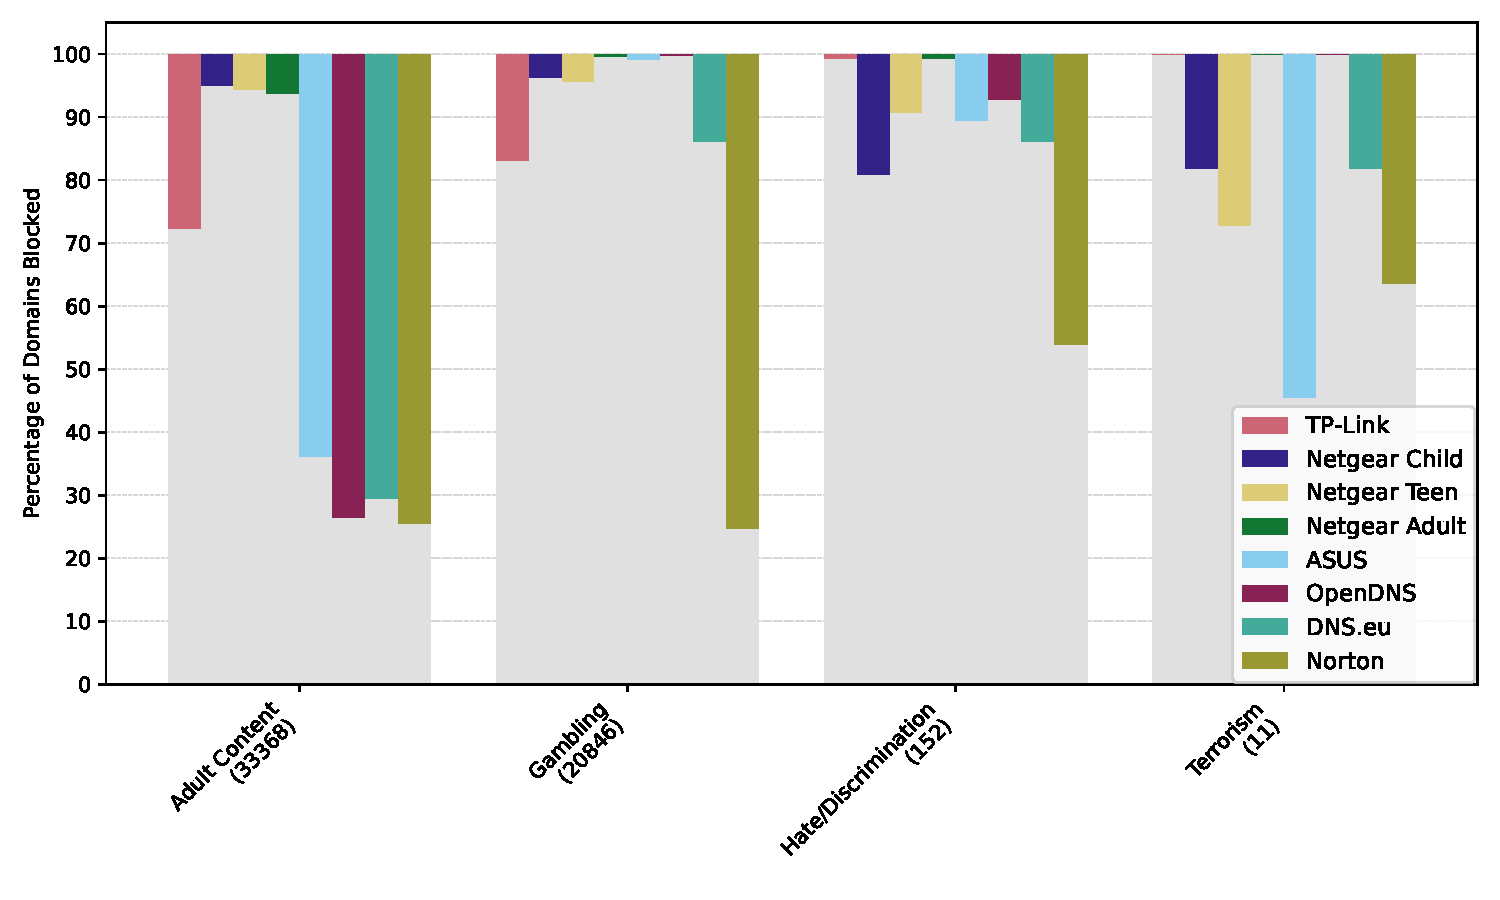
\includegraphics[width=0.85\columnwidth]{Images/Results/blocked_by_category.pdf}
    \caption{Percentage of domains blocked in four core sensitive categories: Adult Content, Gambling, Hate/Discrimination, and Terrorism.}
    \label{fig:blocked_by_category}
\end{figure}
\fi
%\textcolor{red}{Norton, DNS.eu, and OpenDNS consistently demonstrate the highest blocking rates, exceeding 70\% in Adult Content and Gambling, and maintaining strong blocking levels in Hate/Discrimination and Terrorism.
%ASUS shows strong filtering of Adult Content (63.8\%) but drops off sharply in the other categories, suggesting a narrow focus in the blocking policy.
%Netgear, even when using the Child setting, performs poorly across the board, blocking less than 6.5\% in any of the four categories.
%This is particularly problematic for Hate/Discrimination and Terrorism, which receive almost no attention. 
%Notably, while the Child setting is the most restrictive in terms of total domains blocked, it is not the most effective at blocking Adult Content or Gambling. 
%In fact, the Teen setting blocks slightly more Adult Content (5.6\%) than the Child setting (5.0\%), and the Adult setting blocks more Gambling (6.3\%) than both. 
%This pattern, opposite of what would be expected logically, suggests that the Child setting may apply broader but less targeted restrictions, failing to prioritize the most sensitive types of content.
%In contrast, the Teen and Adult settings appear to focus more narrowly on specific high-risk categories.
%However, the overall blocking rates remain low across all three settings, indicating that none of the Netgear configurations offer strong protection for these high-risk categories.
%As mentioned before TP-Link, guided solely by keyword matching, performs surprisingly well in Adult Content (27.7\%) and moderately in Gambling (16.9\%), but completely fails to capture Hate/Discrimination and Terrorism, where associated terms are unlikely to appear in domain names.
%It is important to note that the Terrorism category is very small (only 11 domains), so even slight differences in absolute blocking result in large percentage differences.
%Results regarding that category should be interpreted with caution.}




\begin{figure}[htbp]
    \centering
    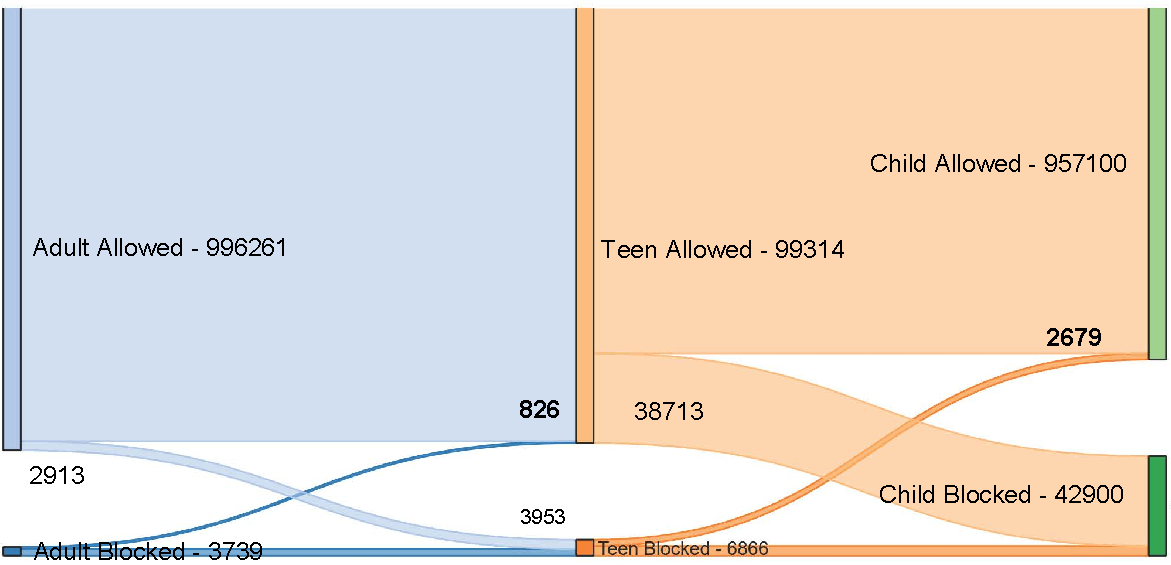
\includegraphics[width=0.95\columnwidth]{Images/Results/bokeh_plot.pdf}
    \caption{Domain Blocking Decisions Across Netgear's Child, Teen, and Adult configurations.}
    \label{fig:netgear_sankey}
\end{figure}

Figure~\ref{fig:netgear_sankey} shows the flow of domain blocking across the three Netgear’s parental control settings. 
Each column represents one of these settings, while the edges illustrate how domains are handled across different parental control levels.
At the Adult level, 3,739 domains are blocked, and 996,261 are allowed. Of the 3,739 domains blocked at the Adult level, most (2,913) remain blocked in the Teen setting, but 826 domains are unexpectedly allowed in Teen despite being blocked in Adult, which contradicts the expected progression from stricter to more permissive filtering.
Additionally, 6,866 domains are blocked in the Teen setting. This includes 2,913 domains that were already blocked in the Adult setting, as well as 3,953 domains that were allowed in the Adult setting but are now blocked in the Teen setting.
At the Child level, most of the domains that were blocked in the Teen setting are still blocked, but 2,679 domains that were previously blocked in Teen are now allowed, indicating that the Child setting fails to block content that the supposedly more permissive Teen level restricted.
Additionally, 38,713 domains transition from ``Teen Allowed''  to ``Child Blocked'' , and 957,100 domains remain allowed throughout, which are expected transitions given the increasing strictness of the settings.
%While the overall beahaviour seems coehrent, if lackluster, with a relatively low number of blocked domains in the Child settings that become smaller as we move towards the adul setting, the analysis of the individual domains reveals issues.
%These inconsistencies suggest that each configuration is applying independent filtering logic, with contradicting results, rather than forming a coherent, tiered policy structure.
The blocking logic appears inconsistent, suggesting that each configuration is applying its own filtering criteria, rather than following a coherent, tiered policy. This leads to contradictions among the different settings.
%\todo[inline]{how do i go back from this more specific analysis to the generic upsetplot?}
%After examining internal consistency within a single system, we now shift focus to how the various parental control tools compare. 
%To capture patterns of overlap and divergence in their blocking behavior, we use an UpSet plot.

\begin{figure}[htbp]
    \centering
    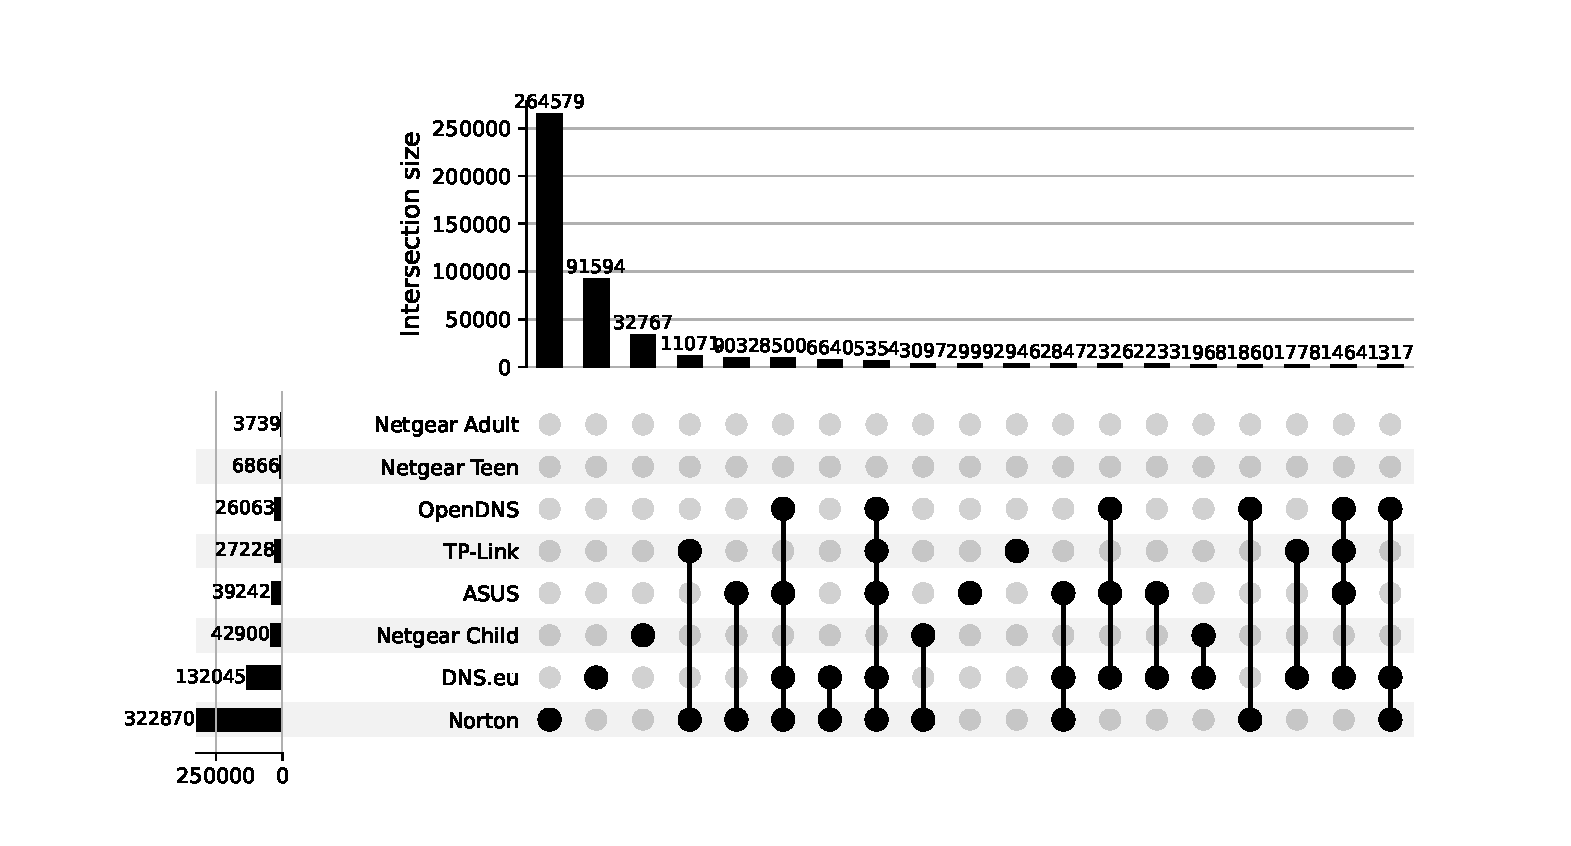
\includegraphics[width=0.95\columnwidth]{Images/Results/upset_blocked_domains_over300.pdf}
    \caption{Overlap in Blocked Domain Across Parental Control Solutions}.
    \label{fig:upset_plot}
\end{figure}

Figure~\ref{fig:upset_plot} presents an UpSet plot showing the intersection of blocked domains across all parental control systems analyzed in this study. We show only intersections containing more than 300 domains for better visibility. Netgear Adult is the only exclusive set not represented in this graph, due to its small size (21).
Each bar represents a group of domains blocked by the combination of systems indicated by the dots below. If a column contains a single dot, it corresponds to the set of domains blocked exclusively by the associated parental control system.
The largest set (264,579) consists of domains blocked only by Norton, highlighting it as the most restrictive tool among those measured.
DNS.eu follows with 91,594 blocked domains exclusively by its filtering system.
The distinctiveness of these exclusive sets highlights how these two tools enforce restrictions more independently and strictly than the others.
Most of the largest intersections involve Norton, which is expected, as it has the largest number of blocked domains.
Notably, Netgear Child, Teen and Adult, rarely overlap, further reflecting the inconsistent blocking behaviors observed in the previous analysis.
Although too small to be clearly visible in the plot, only 205 domains are blocked by all eight parental control solutions, illustrating the lack of alignment across tools and the absence of a unified approach to blocking content.

\textit{Key takeaway: The majority of solutions perform better with adult content domains than other sensitive categories. However, over-blocking in non-sensitive categories is often present. Additionally, more restrictive settings do not automatically mean safer blocking and can lead to inconsistency.}

%\todo[inline]{Antonia: Do we need the following part?}

